\documentclass[11pt,a4paper]{article}

\usepackage[margin=2cm,vmargin=2.5cm,headheight=15.4pt]{geometry}
\usepackage{frenchmath}
\usepackage{xcolor}
\usepackage{amsmath,amssymb}
\usepackage{graphicx}
\usepackage{tikz}
\usetikzlibrary{decorations.pathreplacing}
\usepackage{hyperref}

\setlength\parindent{0pt}
\everymath{\displaystyle}

\hypersetup{
  pdftitle={PGCD : une formule explicite},
  pdfauthor={F. LALLEMAND},
  colorlinks=true,
  linkcolor=blue,
  urlcolor=blue,
  citecolor=blue
}


\title{PGCD : une formule explicite}
\author{F. LALLEMAND}
\date{2026-04-24}
\begin{document}
\maketitle


Un ami m'a récemment fait découvrir une formule étonnante : il s'agit
d'une formule explicite pour calculer le PGCD (Plus Grand Commun
Diviseur) de deux nombres entiers \(a\) et \(b\). La formule est la
suivante, pour tous \((a,b) \in \mathbb{N}^2\) :

\[\boxed{pgcd(a,b) = a + b - ab + 2 \sum _{j=1}^{b-1} \left\lfloor \frac{aj}{b} \right\rfloor}\]

où \(\lfloor x \rfloor\) désigne la partie entière de \(x\).

Cette formule est inhabituelle, car on a l'habitude de calculer le PGCD
plutôt à l'aide d'un processus itératif, comme l'algorithme d'Euclide ou
à l'aide de la décomposition en facteurs premiers.

Je vais en donner une démonstration très visuelle et amusante.

Considérons, dans un repère orthonormé \((O, \vec{i}, \vec{j})\) du
plan, la droite d'équation \(y = \dfrac{a}{b}x\) et les points du plan
de coordonnées entières situés dans le rectangle \([0,b] \times [0,a]\).

Il est clair que ce rectangle contient exactement \((a+1)(b+1)\) points à
coordonnées entières et que ceux-ci sont répartis de façon symétrique de
part et d'autre de la droite \(y = \dfrac{a}{b}x\).

% figure d'exemple avec b=5 (en abscisse) et a=3 (en ordonnée)
\begin{figure}[h]
  \centering
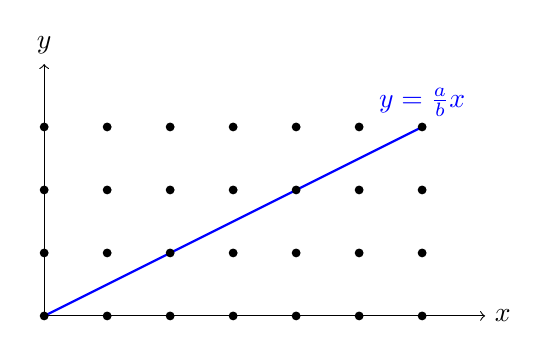
\begin{tikzpicture}[scale=0.8]
  % axes
  \draw[->] (0,0) -- (7,0) node[right] {$x$};
  \draw[->] (0,0) -- (0,4) node[above] {$y$};
  % droite y = (a/b)x
  \draw[thick,blue] (0,0) -- (6,3) node[above] {$y = \frac{a}{b}x$};
  % points à coordonnées entières
  \foreach \x in {0,...,6} {
    \foreach \y in {0,...,3} {
      \fill (\x,\y) circle (2pt);
    }
  }
\end{tikzpicture}
\caption{$a=3$, $b=6$, points à coordonnées entières dans le rectangle}
\end{figure}

Notons $N$ le nombre de points à coordonnées entières situés dans le rectangle (au sens large), on a alors : 

\[N = (a+1)(b+1) = ab + a + b + 1\]

Exploitons maintenant la symétrie de la figure pour obtenir une autre expression de $N$. Pour cela, nous allons dénombrer les points à coordonnées entières situés au-dessous (au sens large) de la droite \(y = \dfrac{a}{b}x\) (c'est-à-dire les points \((x,y)\) à coordonnées entières tels que \(y \leqslant \dfrac{a}{b}x\)).

Par définition de la partie entière d'un réel, nous savons que, pour tout $y\in\mathbb{R}$, $y\geqslant 0$, on a :
\[0 \leqslant \lfloor y \rfloor \leqslant y < \lfloor y \rfloor + 1\]

On en déduit que, pour tout entier $j$ tel que $0 \leqslant j \leqslant b$, le nombre de points d'abscisse $j$ situés au-dessous de la droite \(y = \dfrac{a}{b}x\), au sens large, est égal à \(\left\lfloor \dfrac{aj}{b} \right\rfloor + 1\) : on ajoute 1 pour tenir compte du point d'abscisse $j$ situé sur l'axe des abscisses.

% figure mettant en évidence les points d'abscisse j=4 en encadrant la colonne en orange
\begin{figure}[h]
  \centering
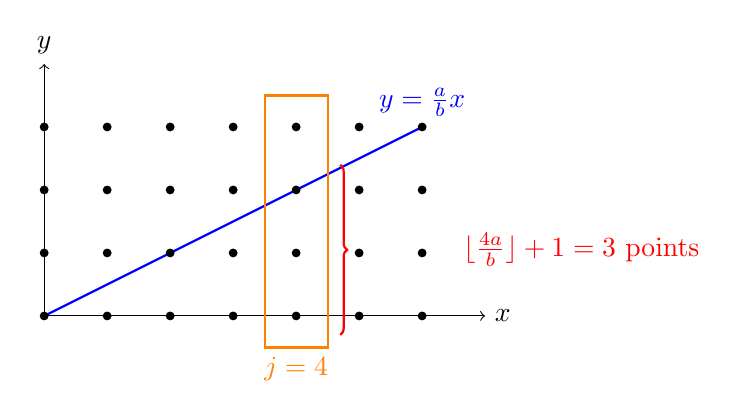
\begin{tikzpicture}[scale=0.8]
  % axes
  \draw[->] (0,0) -- (7,0) node[right] {$x$};
  \draw[->] (0,0) -- (0,4) node[above] {$y$};
  % droite y = (a/b)x
  \draw[thick,blue] (0,0) -- (6,3) node[above] {$y = \frac{a}{b}x$};
  % points à coordonnées entières
  \foreach \x in {0,...,6} {
    \foreach \y in {0,...,3} {
      \fill (\x,\y) circle (2pt);
    }
  }
  % encadrement de la colonne d'abscisse j=4
    \draw[thick,orange] (3.5,-0.5) rectangle (4.5,3.5);
  \node[orange,below] at (4,-0.5) {$j=4$};
  % accolade mettant en évidence les points sous la droite
  \draw[thick,red,decorate,decoration={brace,mirror}] (4.7,-0.3) -- (4.7,2.4);
  \node[red,right] at (6.5,1.05) {$\lfloor\frac{4a}{b}\rfloor + 1 =3 \text{ points}$};
\end{tikzpicture}
\caption{$a=3$, $b=6$, points d'abscisse 4}
\end{figure}

En sommant sur tous les entiers $j$ tels que $0 \leqslant j \leqslant b$, on trouve que le nombre de points à coordonnées entières situés au-dessous de la droite \(y = \dfrac{a}{b}x\) (au sens large) est égal à :

\[\sum _{j=0}^{b} \left( \left\lfloor \frac{aj}{b} \right\rfloor + 1 \right) = (b+1) + \sum _{j=0}^{b} \left\lfloor \frac{aj}{b} \right\rfloor\]

Remarquons que lorsque $j=0$, on a $\left\lfloor \frac{aj}{b} \right\rfloor = 0$, et que lorsque $j=b$, on a $\left\lfloor \frac{aj}{b} \right\rfloor = a$. La somme précédente peut donc être réécrite de la manière suivante :

\[(b+1) + \sum _{j=0}^{b} \left\lfloor \frac{aj}{b} \right\rfloor = (b+1) + a + \sum _{j=1}^{b-1} \left\lfloor \frac{aj}{b} \right\rfloor\]

En utilisant la symétrie de la figure, on en déduit que le nombre $N$ de points à coordonnées entières dans le rectangle est égal à deux fois le nombre de points situés au-dessous de la droite \(y = \dfrac{a}{b}x\) (au sens large),  en prenant garde à \textbf{ne pas compter deux fois les points situés sur la droite \(y = \dfrac{a}{b}x\)} ! Notons provisoirement $\delta$ le nombre de points à coordonnées entières situés sur la droite \(y = \dfrac{a}{b}x\), on a alors :

\[N = 2 \left( (b+1) + a + \sum _{j=1}^{b-1} \left\lfloor \frac{aj}{b} \right\rfloor \right) - \delta\]

% arranger ci-dessous

Il ne reste plus qu'à calculer $\delta$. Un point à coordonnées entières de la forme \((x,y)\) est situé sur la droite \(y = \dfrac{a}{b}x\) si et seulement si \(y = \dfrac{ax}{b}\), c'est-à-dire si et seulement si \(b \mid ax\).

Soit $d=pgcd(a,b)$, il existe alors des entiers $a'$ et $b'$ tels que $a = da'$ et $b = db'$, avec $pgcd(a',b')=1$. La condition \(b \mid ax\) est alors équivalente à la condition \(db' \mid da'x\), c'est-à-dire à la condition \(b' \mid a'x\). Étant donné que $pgcd(a',b')=1$, cela équivaut à la condition \(b' \mid x\) d'après le théorème de Gauss.

On a donc $x=kb'$, avec $0 \leqslant x \leqslant b$, ce qui équivaut à $0 \leqslant k \leqslant d$ : on en déduit que $k$ peut prendre toutes les valeurs entières de $0$ à $d$. Il y a donc exactement $d+1$ points à coordonnées entières situés sur la droite \(y = \dfrac{a}{b}x\), ce qui signifie que $\delta = d + 1 = pgcd(a,b) + 1$.

En reportant cette valeur de $\delta$ dans l'expression de $N$, on trouve que :
\[N = 2 \left( (b+1) + a + \sum _{j=1}^{b-1} \left\lfloor \frac{aj}{b} \right\rfloor \right) - (pgcd(a,b) + 1)\]
En égalant les deux expressions de $N$, on trouve que :
\[(a+1)(b+1) = 2 \left( (b+1) + a + \sum _{j=1}^{b-1} \left\lfloor \frac{aj}{b} \right\rfloor \right) - (pgcd(a,b) + 1)\]

Développons ce qui peut l'être dans l'expression précédente :
\[ab + a + b + 1 = 2b + 2 + 2a + 2 \sum _{j=1}^{b-1} \left\lfloor \frac{aj}{b} \right\rfloor - pgcd(a,b) - 1\]

En réarrangeant les termes, on trouve que :
\[\boxed{pgcd(a,b) = a + b - ab + 2 \sum _{j=1}^{b-1} \left\lfloor \frac{aj}{b} \right\rfloor}\]

Appliquons cette formule pour calculer le PGCD de $a=3$ et $b=6$. On trouve que :
\begin{align*}pgcd(3,6) &= 3 + 6 - 3 \times 6 + 2 \sum _{j=1}^{5} \left\lfloor \frac{3j}{6} \right\rfloor \\
&= 9 - 18 + 2 \left( \left\lfloor \frac{3}{6} \right\rfloor + \left\lfloor \frac{6}{6} \right\rfloor + \left\lfloor \frac{9}{6} \right\rfloor + \left\lfloor \frac{12}{6} \right\rfloor + \left\lfloor \frac{15}{6} \right\rfloor \right) \\
&= -9 + 2 \left( 0 + 1 + 1 + 2 + 2 \right) \\
&= -9 + 2 \times 6 \\
&= -9 + 12 \\
&= 3\end{align*}
Ce qui est bien égal au PGCD de $3$ et $6$.










\end{document}
